


\documentclass[a4paper,11pt]{article}
%\pdfoutput=1 % if your are submitting a pdflatex (i.e. if you have
             % images in pdf, png or jpg format)
\usepackage{jheppub} % for details on the use of the package, please
                     % see the JHEP-author-manual
\usepackage[T1]{fontenc} % if needed
\usepackage{booktabs}

\usepackage{slashed}
%\usepackage{subfigure}
\usepackage{xspace}
\usepackage{booktabs}
%% %simple case: 2 authors, same institution
%% \author{A. Uthor}
%% \author{and A. Nother Author}
%% \affiliation{Institution,\\Address, Country}

\begin{document}
\title{\boldmath Status of the Fittino-ScyNet-SModelS Project}

\author[a]{Federico Ambrogi}
\affiliation[a]{University of Vienna, Institut  f\"ur Meteorologie und Geophysik,  Althanstrasse 14 (UZA II), 1090 Wien}
% e-mail addresses: one for each author, in the same order as the authors\emailAdd{federico.ambrogi@oeaw.ac.at}
\emailAdd{federico.ambrogi88@gmail.com}

\maketitle




\newcommand{\MG}{\texttt{MadGraph5\_aMC@NLO}}

\newcommand{\jmet}{ $3jet+E_T^{miss}$ }

\newcommand{\SMO}{ \texttt{SModelS}}
\newcommand{\FastLim}{ \texttt{FastLim}}


\section*{Abstract}


\section{Introduction}

This document summarizes the current status of the project.

\subsection{To Clarify}
I am not sure about the meaning of these entries in the results root file:
\begin{itemize}
	\item ("SModelSCalculator\_UnusedModel\_0\_Weight")
	\item ("SModelSCalculator\_UnusedModel\_0\_Bracket") 
	\item ("SModelSCalculator\_UnusedModel\_0\_TxName") 
	\item ("SModelSCalculator\_UnusedModel\_0\_FractionOutsideGrid") 
	\item ("SModelSCalculator\_ConstraintOutsideGrid\_0\_Weight") 
	\item ("SModelSCalculator\_ConstraintOutsideGrid\_0\_Bracket") 
	\item ("SModelSCalculator\_ConstraintOutsideGrid\_0\_Bracket") 
	\item ("SModelSCalculator\_MissingConstraint\_0\_Weight") 
\end{itemize}

\clearpage
\section{Results}
In this Section I summarize briefly the results from the first, preliminary scan of points that Bjorn provided.

\subsection{Mass Distributions}
In Fig. \ref{masses} the distributions of the masses of the scanned points are shown; in particular, all the coloured particles have very large masses exceeding 2 TeV, so that essentially only electroweak productions have reasonable cross sections.
This configuration of mass parameters is very challenging for \SMO~, since basically EMs for squark are produced up to around 1 TeV, and gluino EMs for up to 1.5 TeV (but cross sections should be very small in any case to contribute significantly). 
\\
Concerning the Electroweak simplified models, they are very poorly covered: only TSlepSlep (slepton production and direct decay) and TChiWZ (chargino-neutralino2 production but strictly mass degenerate ) are essentially covered. 

\begin{figure}[!b]
	\centering
	\subfigure
	{ 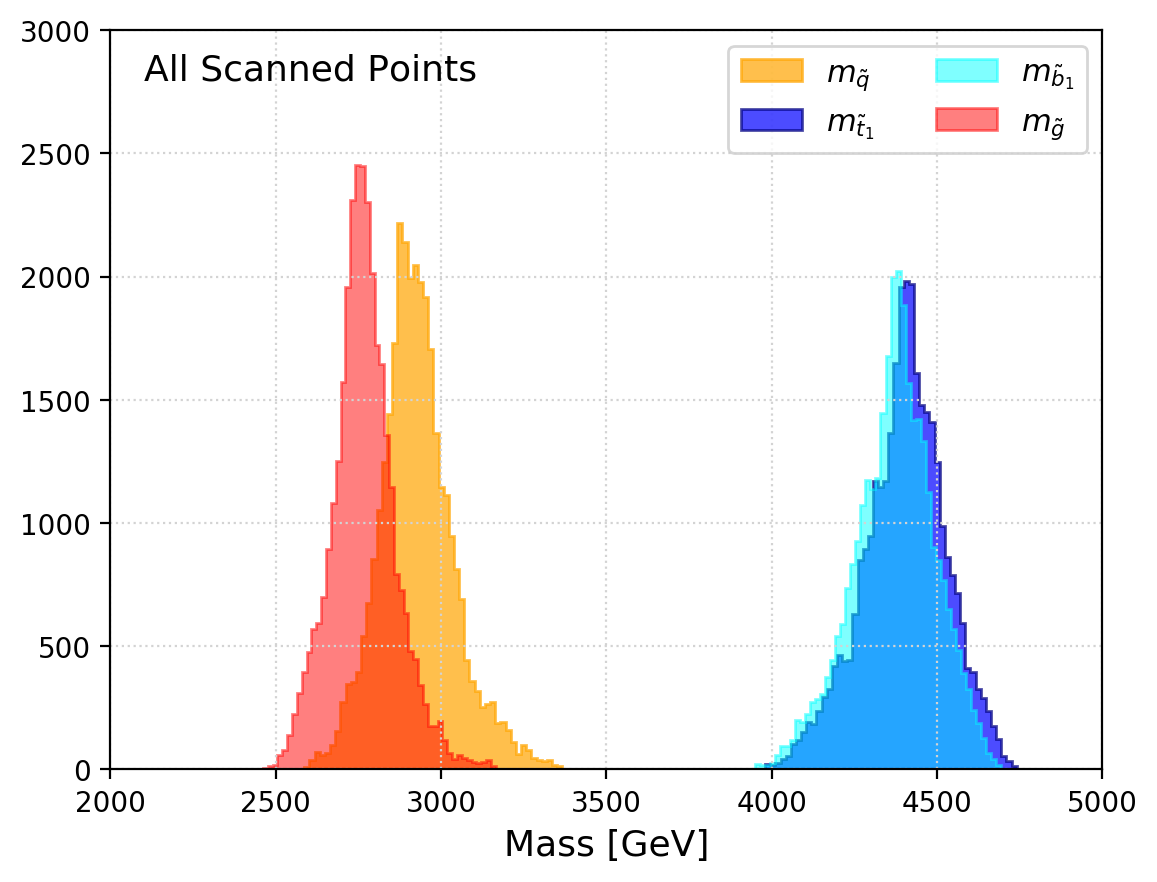
\includegraphics[width=0.49\textwidth]{Fig/Res/Coloured.png}}
	\subfigure
	{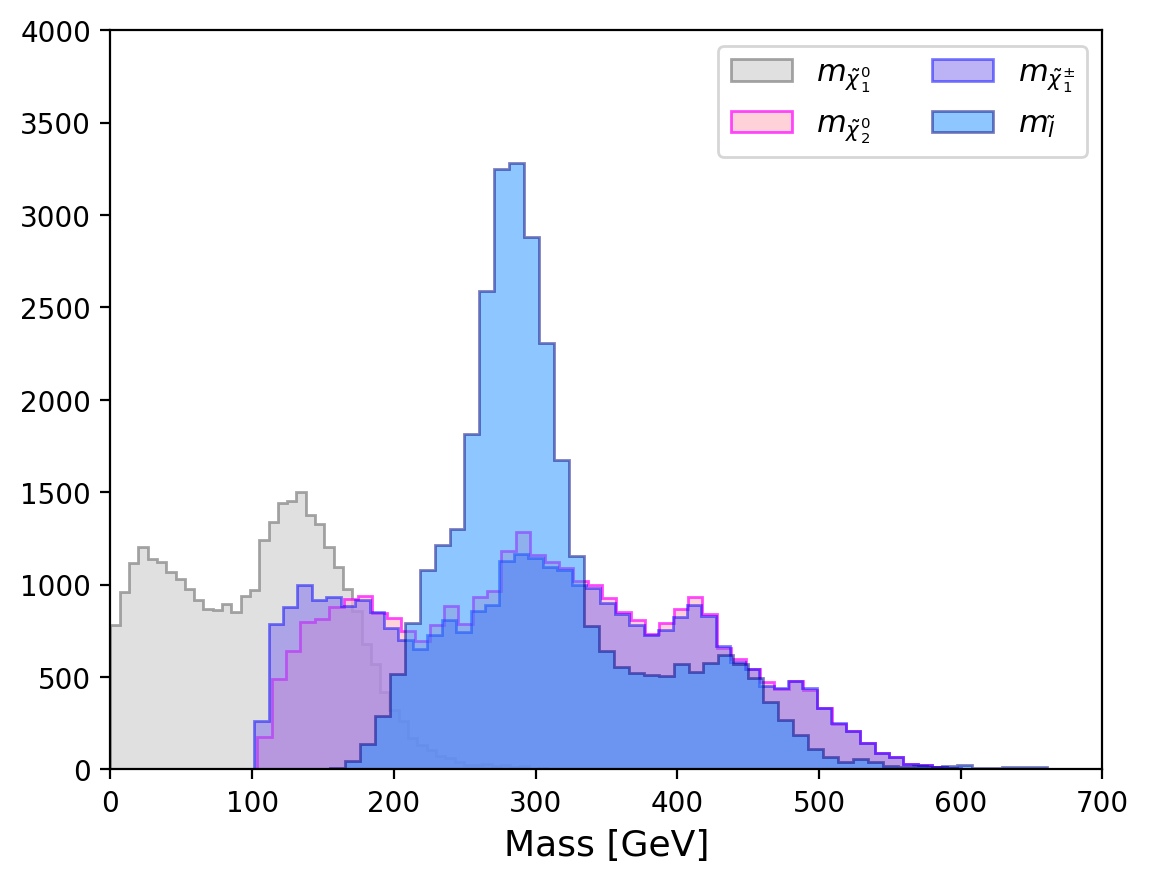
\includegraphics[width=0.49\textwidth]{Fig/Res/EW.png}}
	\subfigure
    {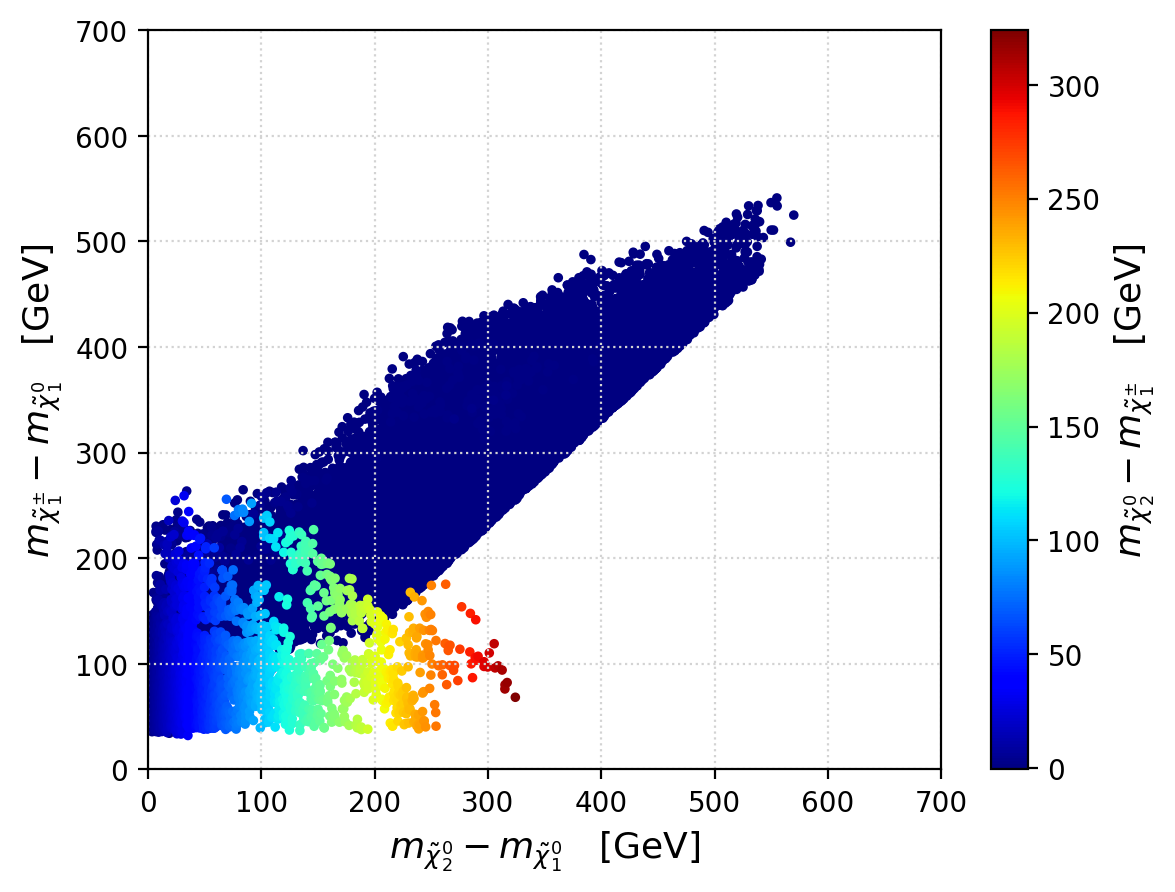
\includegraphics[width=0.49\textwidth]{Fig/Res/Diff_EW.png}}	
    \subfigure
        {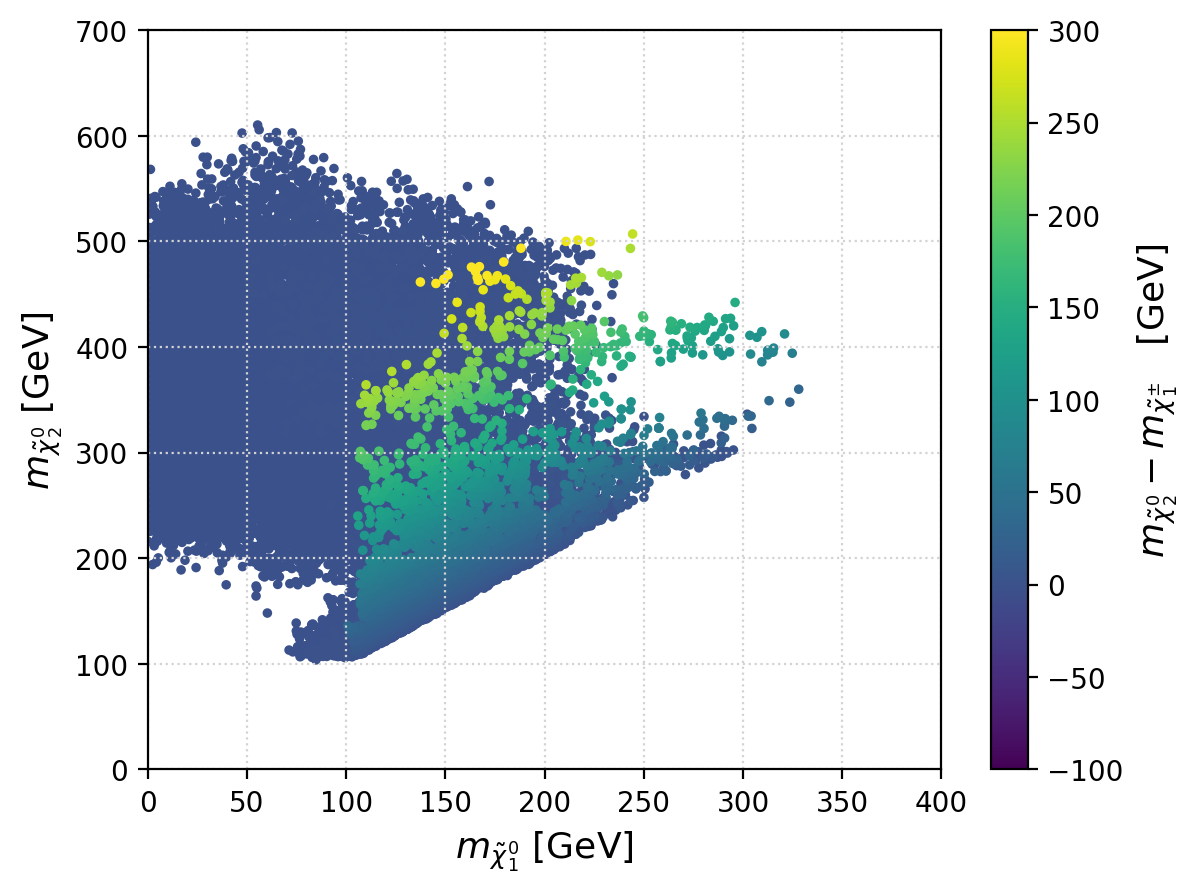
\includegraphics[width=0.49\textwidth]{Fig/Res/Diff_N2_N1_C_EW.png}}	
    
    
	\caption{Distributions of the masses of the SUSY particles of the first set of points.}
	\label{masses}
\end{figure}

\clearpage
\subsection{Missing TxNames and Missing Brackets}
Here I list the most frequent (at least $> 100$ times) missing TxNames and missing brackets, with the largest weight ($\sigma \times BR$) for each point. I am not sure about the interpretation of the two definitions, so I hope Bjorn will clarify this.

\begin{verbatim}
('TChiChipmhiggs_W_', 136)
('TChiChipmZW_WW_', 144)
('TChiChipmqq_W_', 166)
('', 401)
('TChiChipm__', 540)
('TChiChipmmu__', 639)
('TChipChimWoff_Woff_', 950)
('TChiChipm_Woff_', 1341)
('TChiChipmZoff_Woff_', 1569)
('TSnuSnu__', 3249)
('TChiChipm_W_', 3621)
('TChiChi__', 5481)
('TChiChipme__', 8087)
\end{verbatim}

\begin{verbatim}
('[[[W],[W]],[[Z],[W]]]', 160)
('[[[jet,jet]],[[photon]]]', 176)
('[[],[[l,nu]]]', 179)
('[[[W]],[[jet,jet]]]', 184)
('', 401)
('[[],[[W]]]', 1431)
('[[],[[jet,jet]]]', 1648)
('[[[jet,jet]],[[l,nu]]]', 1856)
('[[[W]],[[l,nu]]]', 2124)
('[[],[]]', 4794)
('[[],[[l]]]', 13435)
\end{verbatim}

There are some things that I cannot explain, e.g.
\begin{itemize}
	\item The difference between 'TChiChipme' and the '[[],[[l]]]' constraint? Are those referring to the same topology? \\
	\item Why "TChiChipmmu" is much less frequent than "TChiChipme"? 
	\item What is "TSnuSnu" ?
\end{itemize}



\begin{figure}[!b]
	\centering
	\subfigure
	{ 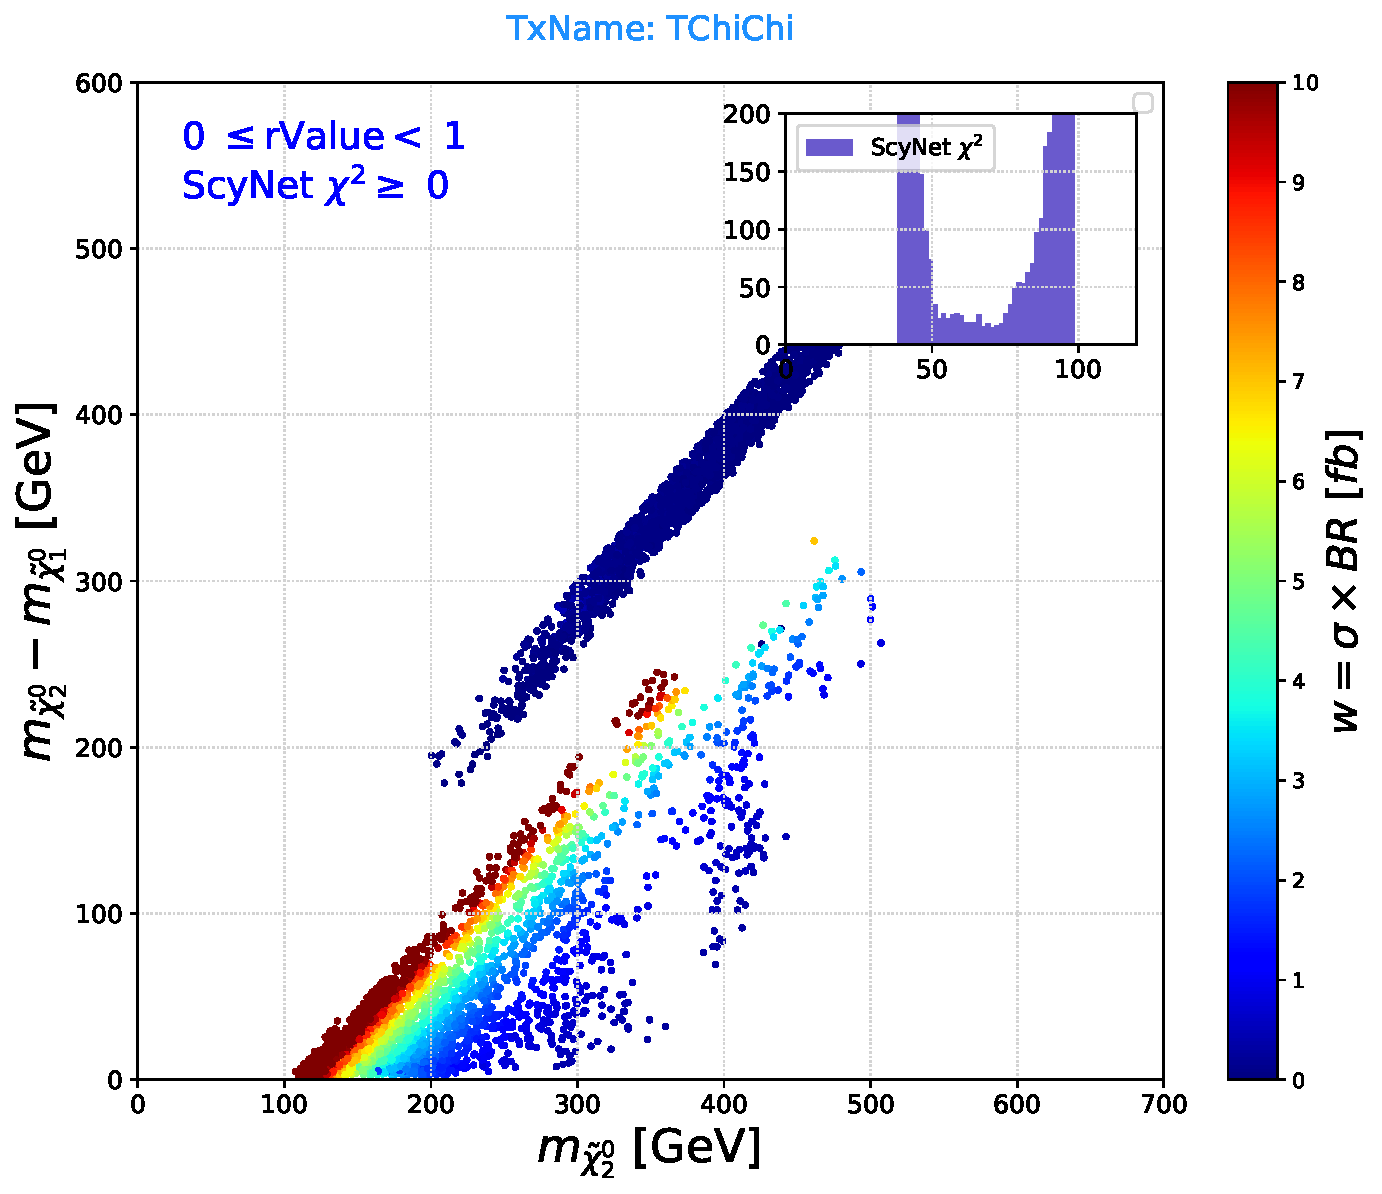
\includegraphics[width=0.49\textwidth]{Fig/Res/Missing_Weights/TChiChi.pdf}}
	\subfigure
	{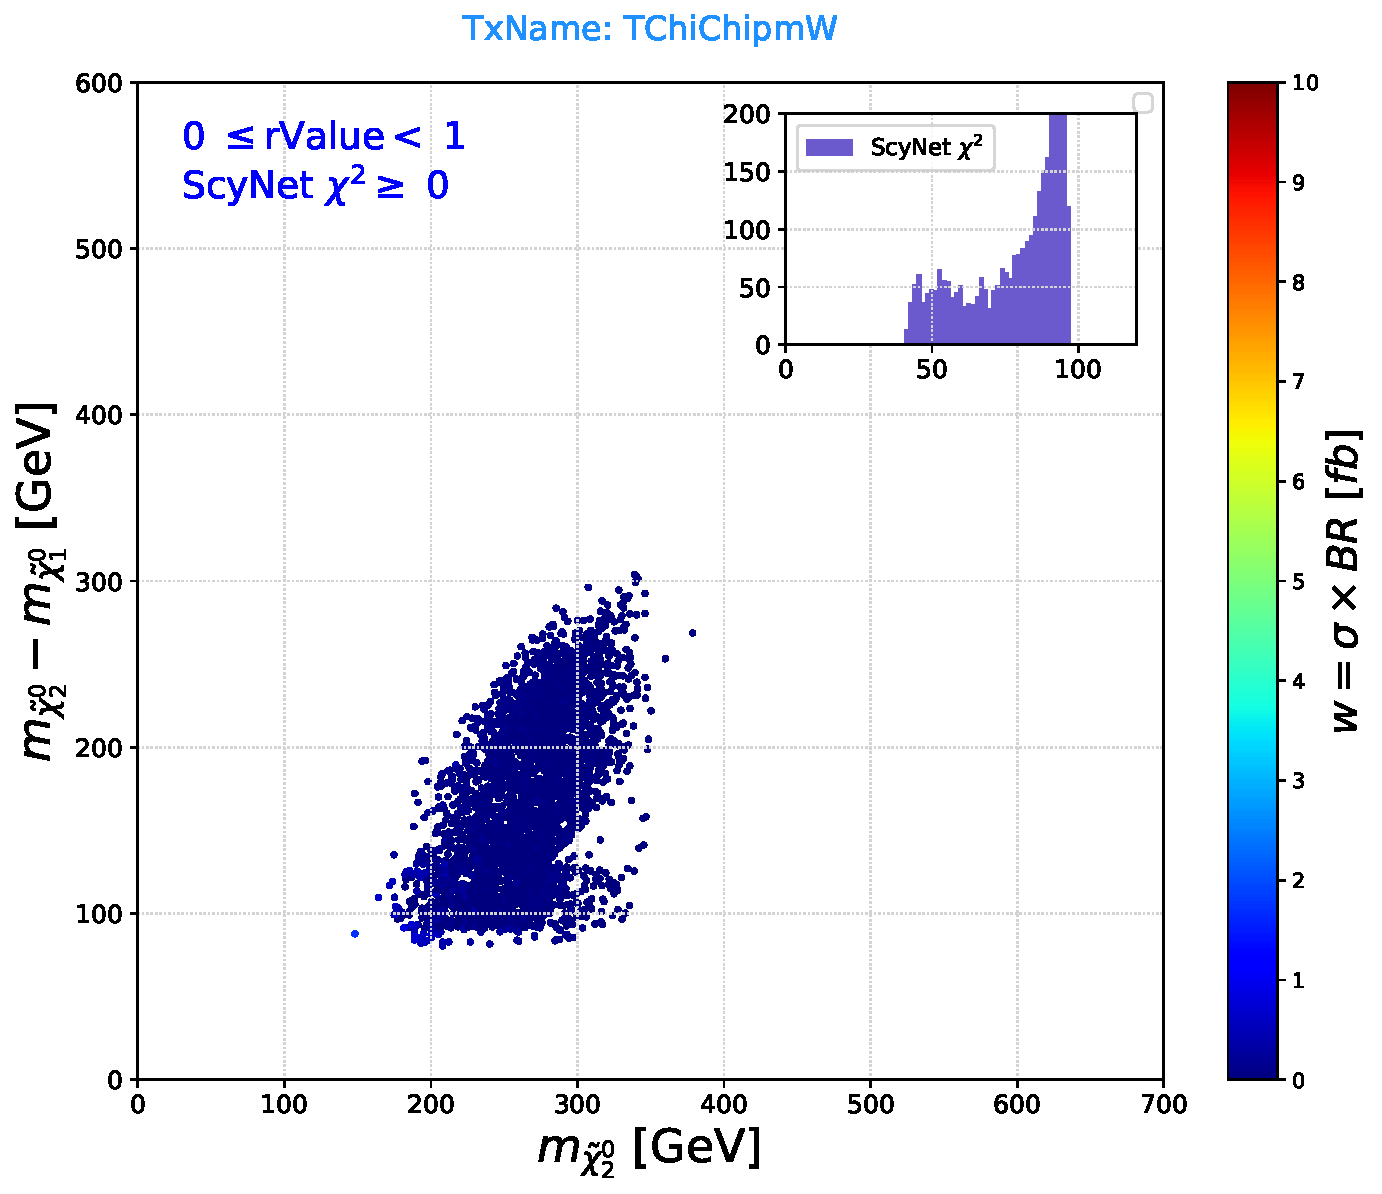
\includegraphics[width=0.49\textwidth]{Fig/Res/Missing_Weights/TChiChipm_W.pdf}}
	\subfigure
	{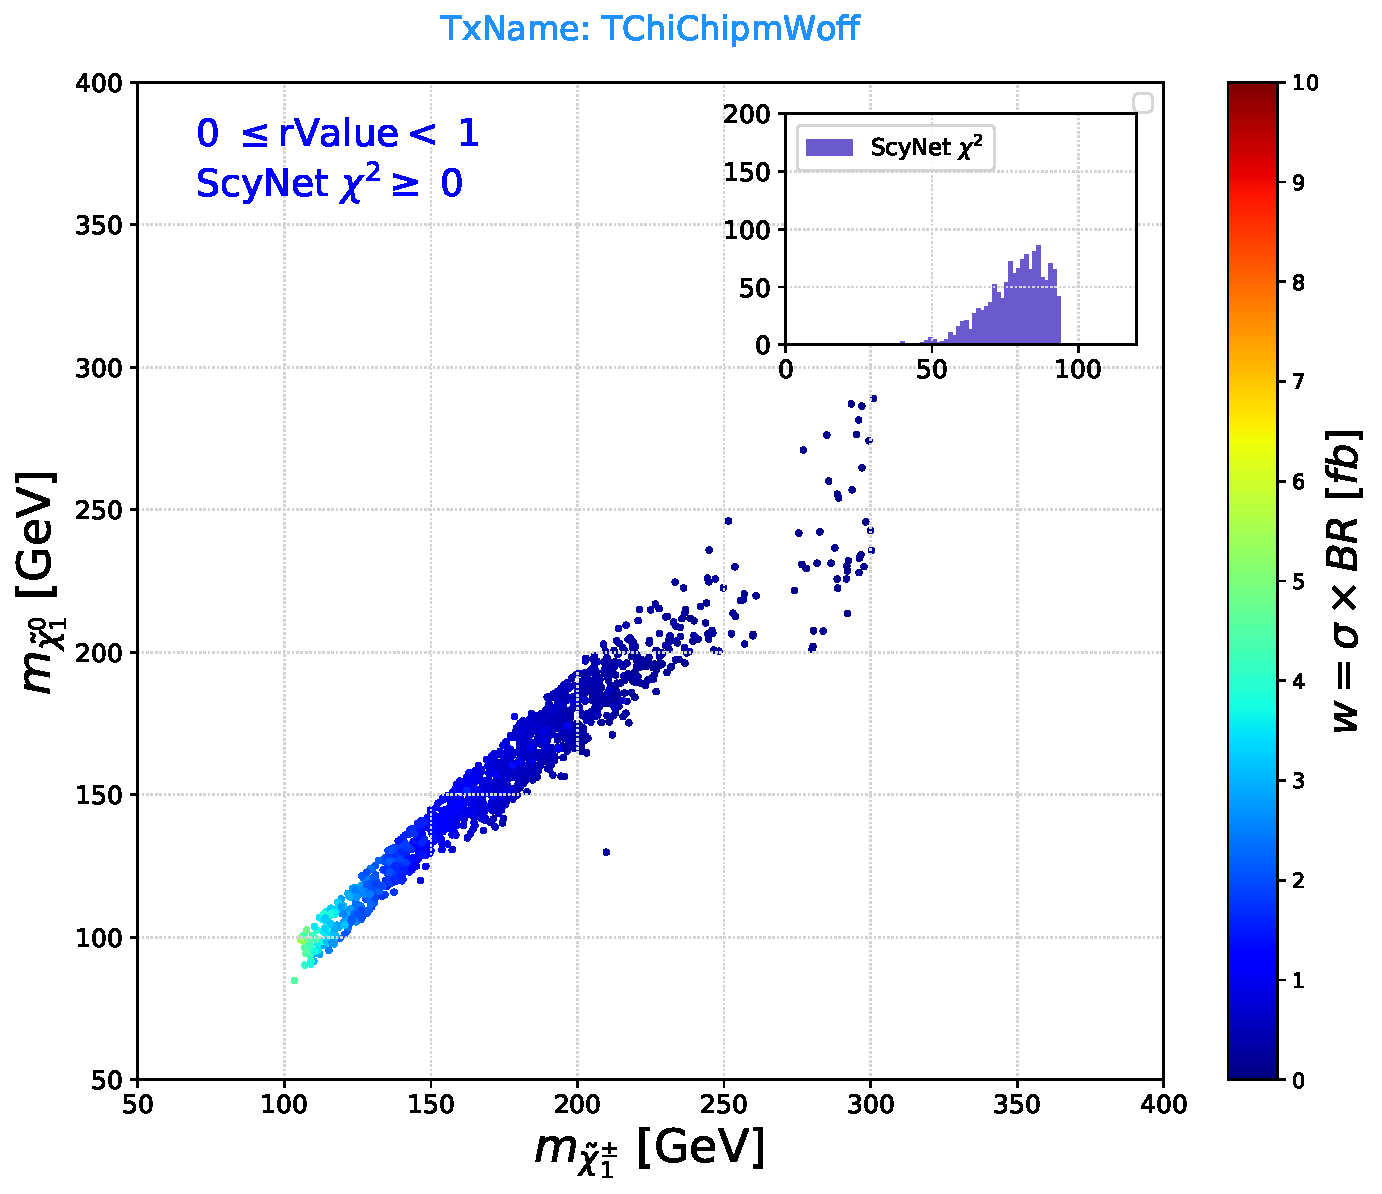
\includegraphics[width=0.49\textwidth]{Fig/Res/Missing_Weights/TChiChipm_Woff.pdf}}	
	\subfigure
	{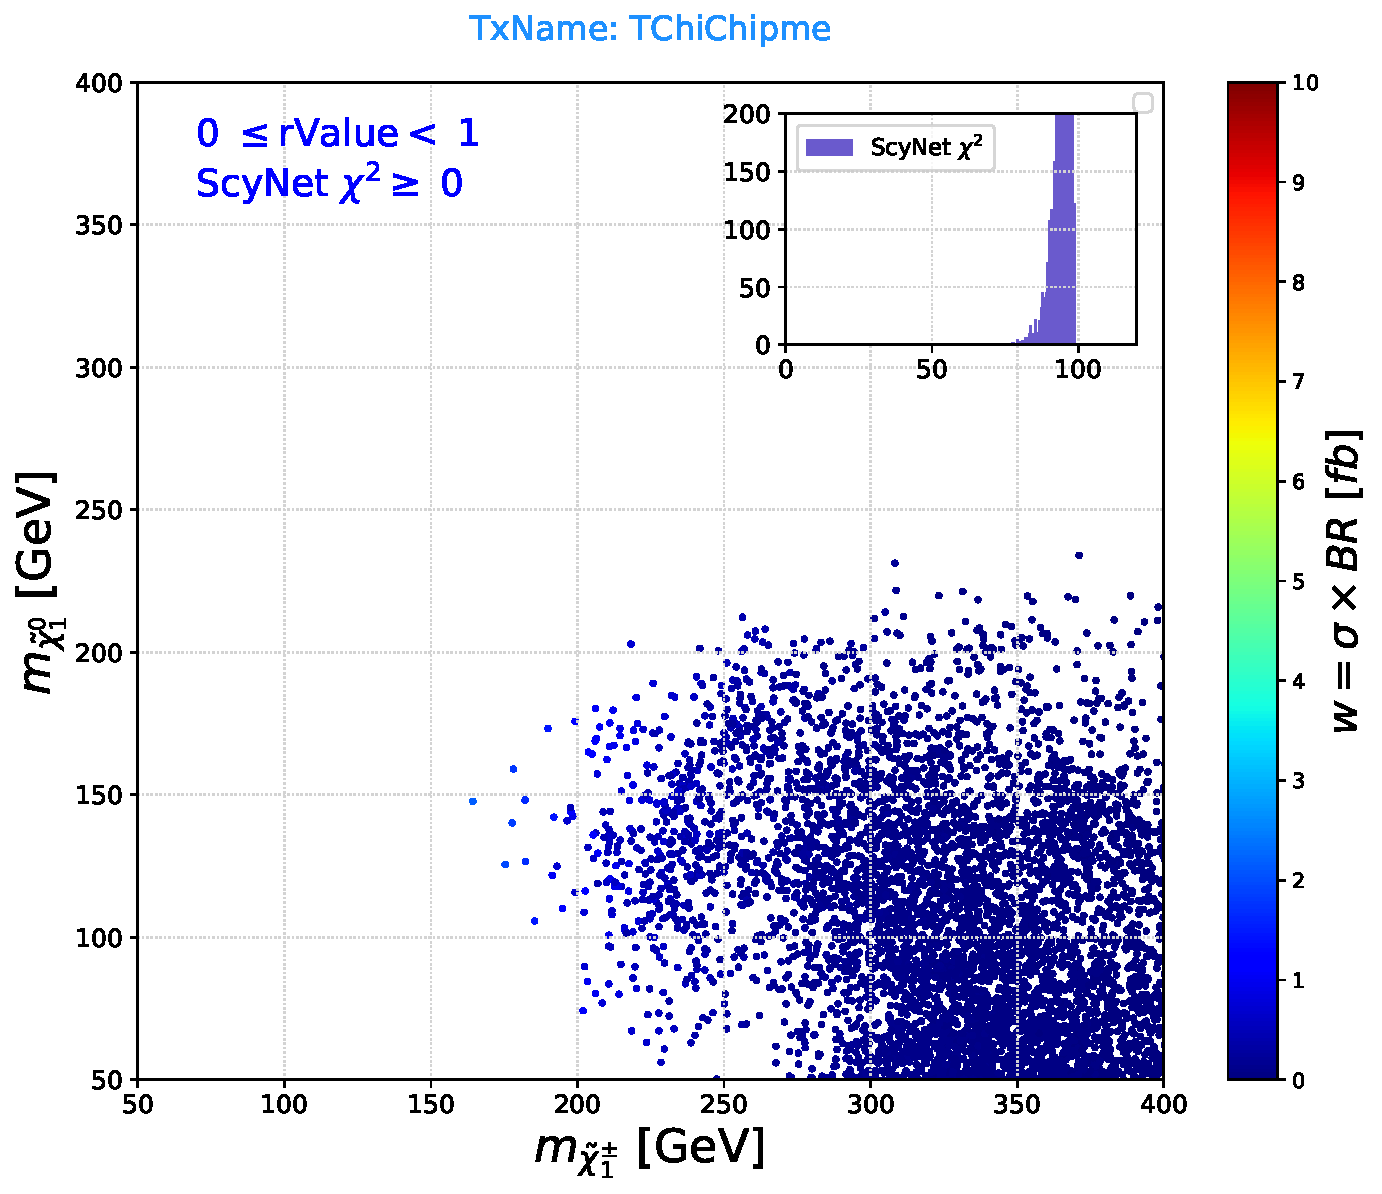
\includegraphics[width=0.49\textwidth]{Fig/Res/Missing_Weights/TChiChipme.pdf}}	
	\subfigure
	{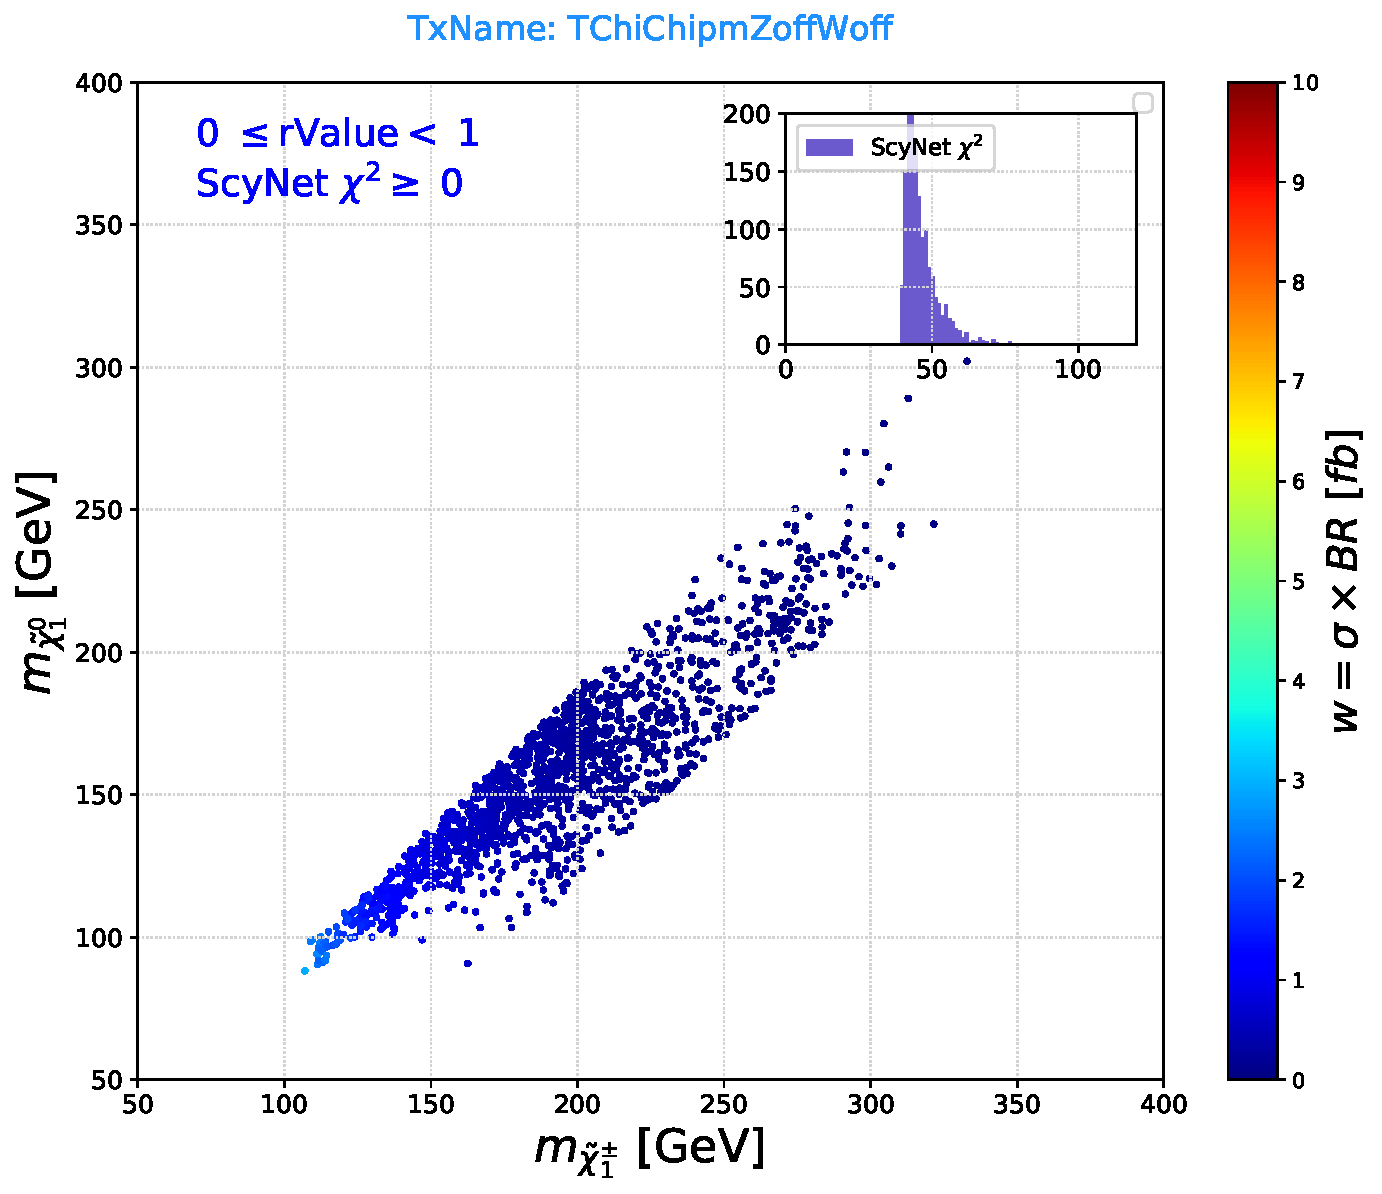
\includegraphics[width=0.49\textwidth]{Fig/Res/Missing_Weights/TChiChipmZoff_Woff.pdf}}	
	\subfigure
	{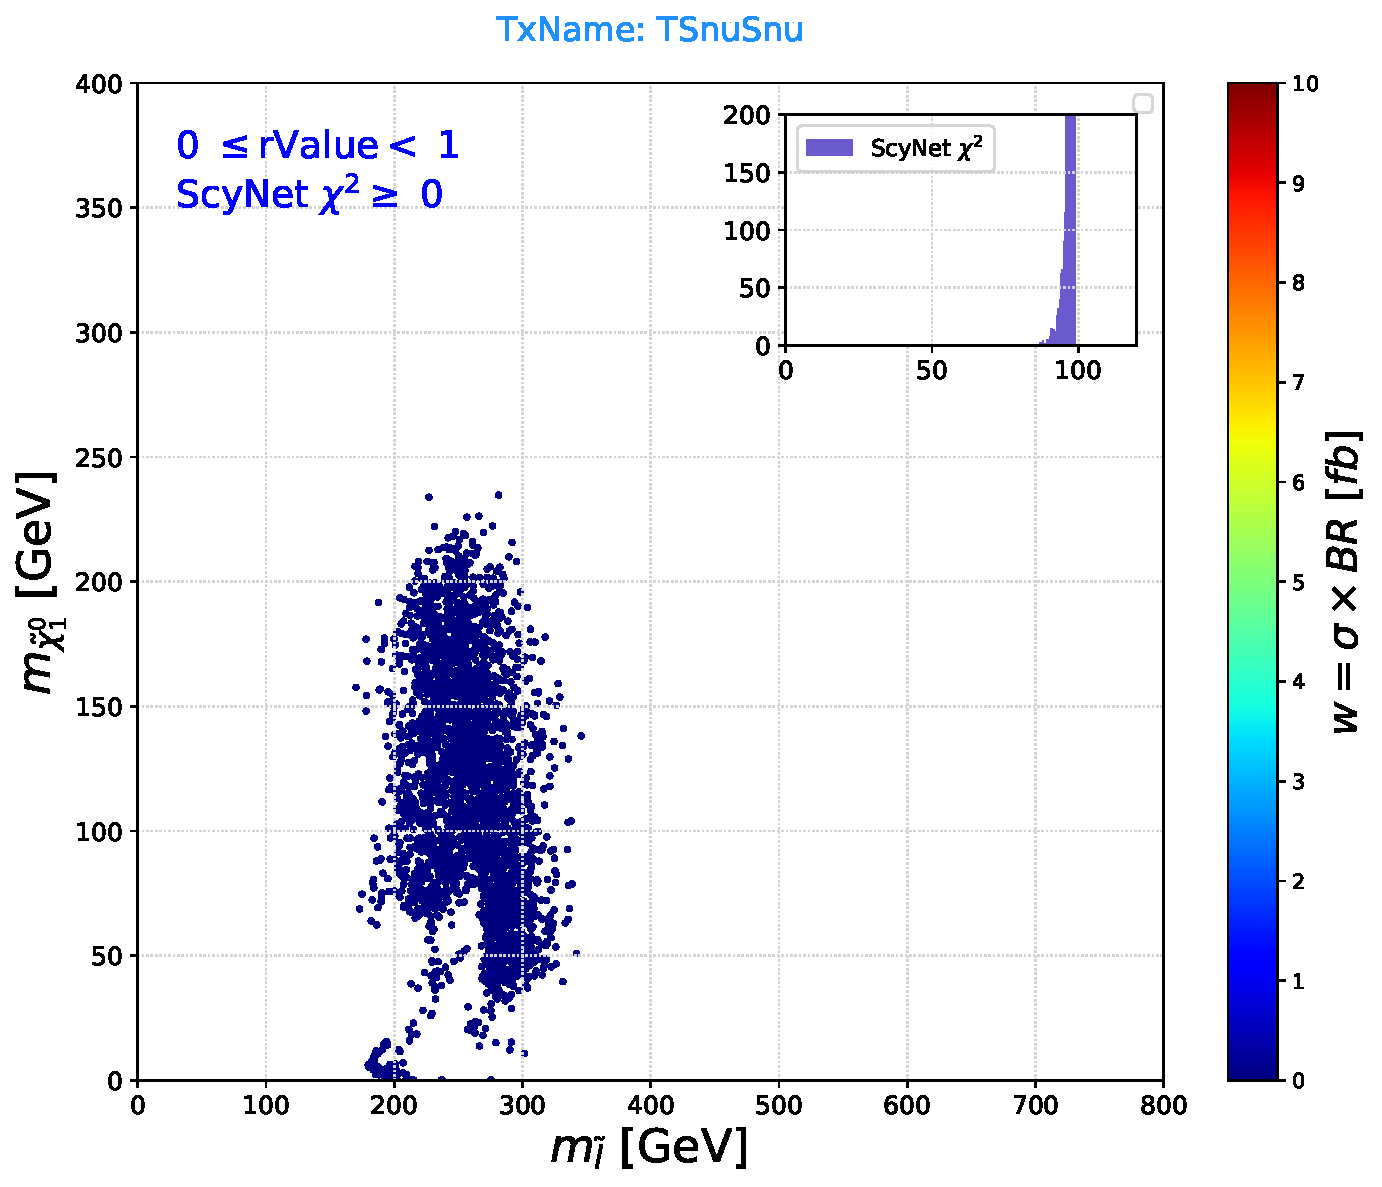
\includegraphics[width=0.49\textwidth]{Fig/Res/Missing_Weights/TSnuSnu.pdf}}	
	
	
	\caption{Weights $\sigma \times BR$ [fb] for the most frequent missing topologies.}
	\label{masses}
\end{figure}




\section{Outside of the grid}

\begin{verbatim}
  [[[jet]],[[jet]]] 6645
  [[[l],[l]],[[l],[nu]]] 5476
  [[[jet,jet]],[[jet,jet]]] 2912
  [[[l,l]],[[l,nu]]] 1754
  [[[W]],[[higgs]]] 1727
  [[[b,b]],[[jet,jet]]] 1356
  [[[l,nu]],[[l,nu]]] 1152
  [[[l],[l]],[[nu],[l]]] 643
  [[[l],[nu]],[[ta],[ta]]] 611
  [[[l],[l]],[[ta],[nu]]] 256
  [[[jet],[W]],[[jet],[W]]] 155
  [[[l],[nu]],[[nu],[l]]] 136
  [[[W]],[[Z]]] 127
\end{verbatim}




\clearpage


\section*{Acknowledgments}
Thanks!
%
\bibliographystyle{JHEP}
\bibliography{references}

\end{document}
